\documentclass[a4paper, 11pt,twoside, leqno]{report}

\usepackage[T1]{fontenc}
\usepackage[utf8x]{inputenc}
\usepackage[greek,english,french]{babel}
\usepackage[babel=true]{csquotes}
\usepackage[top=2.5cm, bottom=2.7cm, left=2.5cm, right=2.5cm]{geometry}
\usepackage{fancyhdr}
\usepackage{graphicx}
\usepackage{amsmath}
\usepackage{soul}
\usepackage{amssymb}
\pagestyle{plain}
\usepackage{amsfonts}
\usepackage{amssymb}
\usepackage{amsthm}
\usepackage{graphicx}
\usepackage{color}
\usepackage{xcolor}
\usepackage{enumerate}
\usepackage{array}
\theoremstyle{plain}
\usepackage{blkarray}
\usepackage{listings}
\usepackage{algorithmicx}
\usepackage{algpseudocode}
\usepackage{algorithm}
\usepackage{lscape}
\usepackage{pdflscape}
\usepackage{eurosym}
\usepackage{hyperref}

\usepackage{caption}
\DeclareCaptionFont{white}{\color{white}}
\DeclareCaptionFormat{listing}{\colorbox{gray}{\parbox{\textwidth}{#1#2#3}}}
\captionsetup[lstlisting]{}

\colorlet{punct}{red!60!black}
\definecolor{background}{HTML}{EEEEEE}
\definecolor{delim}{RGB}{20,105,176}
\colorlet{numb}{magenta!60!black}

%%%%%%%%%%%%%%%%%%%%%%%%%%%%%%%%%%%%%%%%%%%%%%%%%%%%%%%% LISTINGS %%%%%%%%%%%%%%%%%%%%%%%%%%%%%%%%%%%%%%%%%%%%%%%%%%%%%%%%
\definecolor{comment}{rgb}{0.12, 0.38, 0.18 } % adjusted, in Eclipse: {0.25, 0.42, 0.30 } = #3F6A4D
\definecolor{keyword}{rgb}{0.37, 0.08, 0.25}  % #5F1441
\definecolor{string}{rgb}{0.06, 0.10, 0.98} % #101AF9

\lstset{
  columns=flexible, %prevent extra spaces
  rulecolor=\color{black!50},
  backgroundcolor = \color{blue!10},
  numbers=none, % line numbering
  showspaces=false,
  showtabs=false,
  breaklines=true,
  showstringspaces=false,
  breakatwhitespace=false,
  commentstyle=\color{comment},
  keywordstyle=\color{keyword},
  stringstyle=\color{string},
  basicstyle=\ttfamily,
  extendedchars=true,
  emph=[2]{In},
  emphstyle=[2]\color{black!70},
  morecomment=[l][\color{blue}]{Out},
  frame=single,
  frameround=tttt,
  framerule=0.3pt,
  framesep=4pt,
  belowcaptionskip=2.1pt,
  literate={à}{{\`a}}1 {â}{{\^a}}1 %                         letter a
           {À}{{\`A}}1 {Â}{{\^A}}1 %                         letter A
           {ç}{{\c{c}}}1 %                                   letter c
           {Ç}{{\c{C}}}1 %                                   letter C
           {é}{{\'e}}1 {è}{{\`e}}1 {ê}{{\^e}}1 {ë}{{\"e}}1 % letter e
           {É}{{\'E}}1 {È}{{\`E}}1 {Ê}{{\^E}}1 {Ë}{{\"E}}1 % letter E
           {î}{{\^i}}1 {ï}{{\"i}}1 %                         letter i
           {Î}{{\^I}}1 {Ï}{{\"I}}1 %                         letter I
           {ô}{{\^o}}1 %                                     letter o
           {Ô}{{\^O}}1 %                                     letter O
           {œ}{{\oe}}1 %                                     letter oe
           {Œ}{{\OE}}1 %                                     letter OE
           {ù}{{\`u}}1 {û}{{\^u}}1 {ü}{{\"u}}1 %             letter u
           {Ù}{{\`U}}1 {Û}{{\^U}}1 {Ü}{{\"U}}1 %             letter U
  % above is a hack to force UTF8 compatibility (only for french)
}

\lstdefinelanguage{json}{
    basicstyle=\normalfont\ttfamily,
    numbers=left,
    numberstyle=\scriptsize,
    stepnumber=1,
    numbersep=8pt,
    showstringspaces=false,
    breaklines=true,
    frame=lines,
    backgroundcolor=\color{background},
    literate=
     *{0}{{{\color{numb}0}}}{1}
      {1}{{{\color{numb}1}}}{1}
      {2}{{{\color{numb}2}}}{1}
      {3}{{{\color{numb}3}}}{1}
      {4}{{{\color{numb}4}}}{1}
      {5}{{{\color{numb}5}}}{1}
      {6}{{{\color{numb}6}}}{1}
      {7}{{{\color{numb}7}}}{1}
      {8}{{{\color{numb}8}}}{1}
      {9}{{{\color{numb}9}}}{1}
      {:}{{{\color{punct}{:}}}}{1}
      {,}{{{\color{punct}{,}}}}{1}
      {\{}{{{\color{delim}{\{}}}}{1}
      {\}}{{{\color{delim}{\}}}}}{1}
      {[}{{{\color{delim}{[}}}}{1}
      {]}{{{\color{delim}{]}}}}{1},
}

\newcommand{\textcode}[1]{\lstset{
  language=,
  title={{\setlength{\fboxsep}{1pt}\fcolorbox{orange}{yellow!20}{\sffamily\scriptsize
              \textcolor{gray!10}{\_}{#1}\textcolor{gray!10}{\_}}}}
  }
}

\newcommand{\vhdl}{\lstset{
  language=VHDL,
  title={{\setlength{\fboxsep}{1pt}\fcolorbox{orange}{yellow!20}{\sffamily\scriptsize
              \textcolor{gray!10}{\_}VHDL\textcolor{gray!10}{\_}}}}
  }
}
%%%%%%%%%%%%%%%%%%%%%%%%%%%%%%%%%%%%%%%%%%%%%%%%%%%%%%%%%%%%%%%%%%%%%%%%%%%%%%%%%%%%%%%%%%%%%%%%%%%%%%%%%%%%%%%%%%%%%%%%%%%


%\parindent=20pt
\fancypagestyle{plain}{
    % Headers
    \fancyhead[R]{Rapport IA02}
    \fancyhead[L]{Frédéric \textsc{Rouffineau} - Antoine \textsc{Pouillaude}}

    % Footers
    \renewcommand{\footrulewidth}{0.1pt}
    \fancyfoot[C]{Université de Technologie de Compiègne}
    \fancyfoot[LE]{\ifnum\thepage>0 \thepage \fi}
    \fancyfoot[RO]{\ifnum\thepage>0 \thepage \fi}
}

\fancypagestyle{empty}{%
    \renewcommand{\headrulewidth}{0pt} % No sub line
    \fancyhead{} % Empty the header

    \renewcommand{\footrulewidth}{0pt}
    \fancyfoot{}
}

%\setlist[itemize,2]{label={$\bullet$}} % use bullets for nested itemize

% First page
%\newcommand{\presentation}[1]{\vspace{0.3cm}\large{\textbf{#1}}\vspace{0.3cm}\\}
%\newcommand{\presentationLarge}[1]{\vspace{0.3cm}\LARGE{\textbf{#1}}\vspace{0.3cm}\\}

% Overrides chapter (numbered and no-numbered) headings: remove space, display only the title
\makeatletter
  \def\@makechapterhead#1{%
  \vspace*{0\p@}% avant 50
  {\parindent \z@ \raggedright \normalfont
    %\ifnum \c@secnumdepth >\m@ne
    %    \huge\bfseries \@chapapp\space \thechapter
    %    \par\nobreak
    %    \vskip 20\p@
    %\fi
    \interlinepenalty\@M
    \Huge \bfseries \thechapter\quad #1
    \vskip 40\p@
  }}
  \def\@makeschapterhead#1{%
  \vspace*{0\p@}% before 50
  {\parindent \z@ \raggedright
    \normalfont
    \interlinepenalty\@M
    \Huge \bfseries  #1\par\nobreak
    \vskip 40\p@
  }}
\makeatother


%\usepackage{etoolbox}
%\makeatletter
%\patchcmd{\thebibliography}{%
%    \chapter*{\bibname}\@mkboth{\MakeUppercase\bibname}{\MakeUppercase\bibname}}{%
%    \section*{References}}{}{}
%\makeatother
%\DeclareCaptionFont{white}{\color{white}}
%\DeclareCaptionFormat{listing}{\colorbox{black}{\parbox{\textwidth}{#1#2#3}}}
%\captionsetup[lstlisting]{format=listing,labelfont=white,textfont=white}

%\frenchbsetup{StandardLists=true}
%\renewcommand{\labelitemi}{\textbullet}

%\newcommand{\bigO}[1]{\ensuremath{\mathop{}\mathopen{}O\mathopen{}\left(#1\right)}}
%\newcommand{\smallO}[1]{\ensuremath{\mathop{}\mathopen{}o\mathopen{}\left(#1\right)}}

%\title{\textsc{\textbf{Stage TN09 : Assistant ingénieur}}}
%\author{\textbf{Antoine Pouillaude}}

\setcounter{tocdepth}{3}
\begin{document}
    \begin{titlepage}

\vspace*{1.7cm}
\newcommand{\HRule}{\rule{\linewidth}{0.5mm}} % Defines a new command for the horizontal lines, change thickness here

\center % Center everything on the page

%----------------------------------------------------------------------------------------
%	LOGO SECTION
%----------------------------------------------------------------------------------------


\includegraphics[scale=0.45]{logo_UTC.jpg}\\[2.5cm] % Include a department/university logo - this will require the graphicx package
 
%----------------------------------------------------------------------------------------
 
%----------------------------------------------------------------------------------------
%	HEADING SECTIONS
%----------------------------------------------------------------------------------------
\textsc{\Large IA02 : Résolution de Problèmes}\\[0.5cm] % Major heading such as course name
%\textsc{\large Minor Heading}\\[0.5cm] % Minor heading such as course title

%----------------------------------------------------------------------------------------
%	TITLE SECTION
%----------------------------------------------------------------------------------------

\HRule \\[1cm]
{ \huge \bfseries Prolog Chicago Stock Exchange}\\[0.4cm] % Title of your document
\HRule \\[1.5cm]
 
%----------------------------------------------------------------------------------------
%	AUTHOR SECTION
%----------------------------------------------------------------------------------------
\emph{Authors:}\\[0.7cm]
\begin{minipage}{0.4\textwidth}
\begin{flushleft} \large
Antoine \textsc{Pouillaude} \\ % Your name
GI05 Filière SRI
\end{flushleft}
\end{minipage}
~
\begin{minipage}{0.4\textwidth}
\begin{flushright} \large
%%\emph{Supervisor:} \\
Frédéric \textsc{Rouffineau} \\% Supervisor's Name
GI04
\end{flushright}
\end{minipage}\\[3cm]

%----------------------------------------------------------------------------------------
%	LOGO SECTION
%----------------------------------------------------------------------------------------

%\includegraphics[scale=0.3]{logo_metadot.png}\\[1cm] % Include a department/university logo - this will require the graphicx package
 
%----------------------------------------------------------------------------------------

% If you don't want a supervisor, uncomment the two lines below and remove the section above
%\Large \emph{Author:}\\
Université de Technologie de Compiègne\\
Rue Roger Couttolenc\\
60200 Compiègne\\[2cm] % Your name

%----------------------------------------------------------------------------------------
%	DATE SECTION
%----------------------------------------------------------------------------------------

{\large \today}\\[3cm] % Date, change the \today to a set date if you want to be precise

\vfill % Fill the rest of the page with whitespace

\end{titlepage}
\tableofcontents

\chapter{Introduction}

Nous avons eu pour projet, dans le cadre de l'Unité de Valeur IA02 (Résolution de Problèmes et programmation logique), de coder le jeu Chicago Stock Exchange à l'aide du langage Prolog. Il s'agit d'un jeu de plateau pouvant se jouer à 2 joueurs ou plus durant lequel ils vont essayer de maximiser leur profit en vendant et en achetant des denrées alimentaires. 
Afin de simplifier l'implémentation du jeu sous Prolog, nous avons limité le nombre de joueurs à 2. Nous devions également créer une Intelligence Artificielle afin de pouvoir jouer contre l'ordinateur. 

Lors d'un tour de jeu un joueur va déplacer un pion Trader sur des piles de denrées d'au moins 1 et d'au plus 3 piles. Il/elle va alors récolter les deux jetons situés sur le dessus des piles adjacentes du Trader, choisir d'en garder une et d'en jeter une. Jeter une denrée à pour effet de diminuer la valeur en bourse de cette denière. Le joueur avec le stock de plus grande valeur gagne la partie.\\


\section{Modèle}
\noindent Le jeu sera majoritairement modélisé avec une liste représentant l'état de jeu courant. Cette liste sera de la forme : 
\begin{lstlisting}[language=prolog]
[Liste des piles de denrées, État de la bourse, Position du Trader, Réserve du joueur 1, Réserve du joueur 2]
\end{lstlisting}
Les différentes listes qui composent l'état de jeu courant auront les formes indiquées ci-dessous.
\paragraph{Bourse} L'état de la bourse sera modélisé par une liste contenant l'état des différentes denrées côtées à Chicago.
\begin{lstlisting}[language=prolog]
[Etat de la marchandise 1, Etat de la marchandise 2, ..., Etat de la marchandise n]
\end{lstlisting}
L'état d'une marchandise est, quant à lui, une simple liste avec, comme premier élément, le nom de la marchandise en question et en seconde position la valeur en bourse de ladite denrée.
\begin{lstlisting}[language=prolog]
[Marchandise,Valeur en bourse]
\end{lstlisting}
\paragraph{Piles de marchandises.} Le jeu, dans son état initial est composé de 9 piles de 4 denrées différentes. Ces piles sont modélisées par des listes elle-mêmes inclues dans une grande liste contenant toutes les piles.
\begin{lstlisting}[language=prolog]
[[Pile1],[Denrée1,Denrée2,Denrée3,Denrée4],[Pile3],...,[PileN]]
\end{lstlisting}
\paragraph{Trader} La position du Trader sera donnée à l'aide d'un chiffre entre 0 et le nombre de piles contenues dans l'état de jeu courant. 
\paragraph{Réserve}La réserve d'un joueur sera modélisée par une liste avec en tête le nom du joueur en question suivi des denrées que ce joueur possède.
\begin{lstlisting}[language=prolog]
[Nom du joueur, Denrée1,Denrée2,...,DenréeN]
\end{lstlisting}
\paragraph{Coup de jeu}Un coup de jeu doit contenir 4 paramètres : 
\begin{itemize}
	\item le nom du joueur
    \item la valeur du déplacement (1,2 ou 3)
    \item la ressource gardée
    \item la ressource vendue
\end{itemize}
Ces données seront regroupées dans une liste : 
\begin{lstlisting}[language=prolog]
[Nom du joueur, Déplacement,Marchandise gardée,Marchandise vendue]
\end{lstlisting}

\chapter{Principaux prédicats}
\section{Gestion du plateau}
\subsection{Affichage}
Nous avons regroupé le code pour l'affichage du plateau de jeu dans le fichier \textit{game\_{}display.pl}. Le prédicat d'affichage du plateau est le suivant : 
\begin{lstlisting}[language=prolog]
%%%% display_game(+Game_State_To_Be_Displayed)
%% The following predicate displays a game state.
display_game(State) :-
		[Stacks,S,TP,RJ1,RJ2] = State,
		generate_board_from_stock(S,Board),
		display_board(Board),
		nl, nl, nl,
		display_stack(Stacks,TP),
		nl, nl,
		display_players([RJ1,RJ2]),nl,nl,
		evalState(State,Earnings),
		tab(5),display_earnings(Earnings),nl,nl,nl.
\end{lstlisting}

Dans la queue de cette règle on retrouve des appels aux prédicats :
\begin{itemize}
    \item \textit{generate\_{}board\_{}from\_{}stock} qui va, à partir d'un Template d'affichage, générer une liste correspondant au plateau graphique à afficher.  
    \item \textit{display\_{}board} qui affiche le Template généré par la règle précédente.
    \item \textit{display\_{}stacks} qui affiche le dessus de chaque pile de marchandises et le nombre de jetons restant dans ces piles.
    \item \textit{display\_{}players} qui affiche l'état des stocks des différents joueurs.
    \item \textit{display\_{}earnings} qui va afficher le gain en USD des deux joueurs en fonction de leur stock.
\end{itemize}
Au final nous obtenons le rendu suivant : 
\begin{figure}[H]
    \begin{center}
        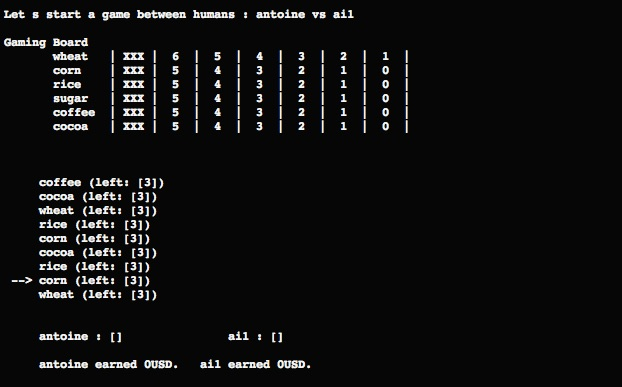
\includegraphics[scale=0.5]{ScreenGamingBoard.jpg}
     \end{center}
     \caption{The result of the gaming board display predicate.}
     \label{fig:gamingboard}
 \end{figure}
     
\subsection{Génération du plateau}
Au début de la partie le plateau doit être généré. Nous faisons appel à la règle de construction \textit{starting\_{}state} :
\begin{lstlisting}[language=prolog]
%%%% starting_state(?State_To_Be_Generated,+Player_1's_Name,+Player_1's_Name)
%% This predicate generates the initial state of the game. 
starting_state(State,NameJ1,NameJ2) :-
		generating_stacks([[wheat,6],[corn,6],[rice,6],[sugar,6],[coffee,6],[cocoa,6]],Stacks,9),
		Bourse = [[wheat,7],[corn,6],[rice,6],[sugar,6],[coffee,6],[cocoa,6]],
		random(0,8,TP),
		State = [Stacks,Bourse,TP,[NameJ1],[NameJ2]].
\end{lstlisting}
Dans ce prédicat nous appelons la règle \textit{generating\_{}stacks}, qui va générer les piles de manière pseudo-aléatoire en faisant appel à la fonction built-in random\/{}3. Par la suite la position initiale du pion Trader est tirée de manière pseudo-aléatoire. 

Il est très intéressant de remarquer le fait que les tirages se font de manière pseudo-aléatoire. À chaque fois le premier état de jeu généré après l'ouverture de l'interpréteur gprolog est toujours le même. 
%\begin{figure}[H]
%    \begin{center}
%        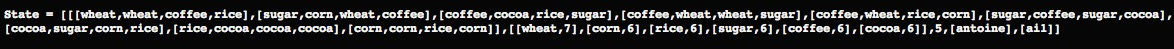
\includegraphics[scale=0.4]{ScreenStartingState.jpg}
%     \end{center}
%     \caption{Premier état généré pseudo-aléatoirement.}
%     \label{fig:startingstate}
% \end{figure}
\section{Déroulement du jeu}
\subsection{Vérification de coup}
Avant de jouer un coup il est important de savoir si celui-ci existe. En effet, si le joueur rentre une mauvaise combinaison de déplacement et de pièces à garder, il faut alors empêcher le joueur de jouer la combinaison. C'est pour cela que nous avons créé le prédicat \textit{is\_{}possible} qui va vérifier si le coup de jeu que l'utilisateur souhaite jouer est conforme à l'état actuel du plateau de jeu.
\newpage

\begin{lstlisting}[language=prolog]
%%%% is_possible(+List_Of_Stacks,+Current_Trader_Position,+Move_The_Player_Wants_To_Make,?Return_Value)
%%% Return_Value = 0 if the move is possible, 1 if the two given element are not on the two stacks adjacent ot the Trader position, 2 if the move applied to the Trader is not in [1,2,3].
%% This predicate will check if a move is possible in the current game configuration.
is_possible(Stacks,TP,[_,Pos,Keep,Sell],ReturnValue):- Pos < 4, Pos >0, !,
		get_indexes(Stacks,TP,Pos,[_,ISup,IInf]),
		nth0(ISup,Stacks,E1),
		nth0(IInf,Stacks,E2),
		test_comb(Keep,Sell,E1,E2,ReturnValue).
is_possible(_,_,_,2).

%%%% test_comb(+The_Element_The_Player_Wants_To_Keep,+The_Element_The_Player_Wants_To_Sell,+One_Of_The_Adjacent_Stack,+The_Other_Adjacent_Stack,?The_Return_Value)
%%% Return_Value = 0 if the two products are on top of the two stacks adjacent to the Trader's position, = 1 otherwise.
%% This rule test if the two elements given in the move are on top of the two adjacent stacks of the Trader stack.
test_comb(Keep,Sell,[Keep|_],[Sell|_],0) :- !.
test_comb(Keep,Sell,[Sell|_],[Keep|_],0) :- !.
test_comb(_,_,_,_,1).
\end{lstlisting}

Ci-dessus nous avons défini deux prédicats pour tester les combinaisons. La règle \textit{test\_{}comb} sert à verifier si l'un des éléments donnés par l'utilisateur est bien sur l'une des piles adjacentes au Trader après déplacement. Le prédicat \textit{get\_{}indexes} va chercher l'index des trois piles concernées par le coup de jeu.

\subsection{Jouer un coup}
Une fois que nous avons vérifié que le coup était viable, il faut maintenant le jouer et modifier l'état de jeu en conséquence. C'est pour cela que le prédicat \textit{play} a été créé. 

\begin{lstlisting}[language=prolog]
%%%% play(+Game_State,+Move_To_Apply,?New_State,-Return_Value)
%% This predicate will update the game state according to the move provided to the function.
play([Stacks,_,_,_,_],_,_,3) :- length(Stacks,Le),Le =< 2, !.
play([Stacks,S,TP,RJ1,RJ2],[Player,Pos,Keep,Sell],NewState,RetValue) :- length(Stacks,Le),Le > 2,is_possible(Stacks,TP,[Player,Pos,Keep,Sell],ExitStatus),
		play_ret([Stacks,S,TP,RJ1,RJ2],[Player,Pos,Keep,Sell],NewState,RetValue,ExitStatus).

%%%% play_ret(+Game_State,+Move_To_Apply,?New_State,-Return_Value,+Value_Returned_By_The_is_possible_Predicate)
play_ret([Stacks,S,TP,RJ1,RJ2],[Player,Pos,Keep,Sell],NewState,0,0) :- !,
		get_indexes(Stacks,TP,Pos,[NTP,ISup,IInf]),
		nth0(ISup,Stacks,E1),
		nth0(IInf,Stacks,E2),
		pop(E1,NE1), pop(E2,NE2),
		update_i(Stacks,ISup,NE1,NTempStacks), update_i(NTempStacks,IInf,NE2,NStacks),
		clean_list_and_update_TP(NStacks,NewStacks,NTP,NTPmod), 
		length(NewStacks,Length), my_mod(NTPmod,Length,NewTP), 
		add_to_player(Player,Keep,RJ1,RJ2,NRJ1,NRJ2),
		member_sec_order_e(S,Sell,Elt), [Name,Value] = Elt, NValue is Value - 1,
		NElt = [Name,NValue], update_e(S,Elt,NElt,NS), 
		NewState = [NewStacks,NS,NewTP,NRJ1,NRJ2].
play_ret([Stacks,S,TP,RJ1,RJ2],_,NewState,ExitStatus,ExitStatus) :- NewState =[Stacks,S,TP,RJ1,RJ2].
\end{lstlisting}

Il y a en fait deux prédicats différents avec le même nom. Le premier va récupérer l'entrée de l'utilisateur ou de l'Intelligence Artificielle et tester si le coup est possible. La règle de test va retourner une valeur en fonction du résultat du test. Si cette valeur est 0 alors le coup est viable et le second prédicat du même nom va alors modifier l'état du jeu en conséquence.

\section{Intelligence artificielle}

Afin de pouvoir jouer seul contre l'ordinateur nous avons créé une intelligence artificielle basée sur l'algorithme de recherche Min-Max avec élagage Alpha/Beta. Cet algorithme va être implémenté par deux prédicats importants.

\subsection{Trouver les coups possibles}
Il faut d'abord trouver tous les coups que l'ordinateur pourra jouer. C'est à cela que sert le prédicat \textit{all\_{}possible\_{}moves}.


\begin{lstlisting}[language=prolog]
%%%% all_possible_moves(+State_Of_The_Game,+Player_Who_Will_Make_The_Move,?Possible_Moves)
%% The following predicate will get all the possible moves that the ai could make.
all_possible_moves([Stacks,_,TP,_,_],Player,PossibleMoves) :- possible_moves(Stacks,TP,Player,[1,2,3],PossibleMoves).


%%%% possible_moves(+Stacks_Of_The_Game,+Trader_Position,+Player_Who_Will_Make_The_Move,+List_Of_Jumps_To_make,?List_Of_Moves)
%% possible_moves will get the list of the moves possible by applying all the jumps given in the fourth parameter. In that game the list should be [1,2,3].
possible_moves(_,_,_,[],[]) :- !.
possible_moves(Stacks,TP,Player,[H|T],ListMoves) :-
		possible_moves(Stacks,TP,Player,T,SListMoves), 
		get_possible_list(Stacks,TP,H,ListProd),
		reverse(ListProd,RevList),
		concat([Player,H],ListProd, TempList),
		concat([Player,H],RevList, TempListRev),
		concat([TempList],[TempListRev],Temp),
		concat(Temp,SListMoves,ListMoves).
\end{lstlisting}

La règle \textit{all\_{}possible\_{}moves} appelle le prédicat \textit{possible\_{}moves} pour tous les déplacements possibles. \textit{possible\_{}moves} va alors retourner toutes les combinaisons de produits gardés et de produits vendus possibles.

Le prédicat \textit{all\_{}possible\_{}moves} va, à la fin, retourner la liste des coups possibles afin, qu'ensuite, l'Intelligence Artificelle puisse déterminer le meilleur coup possible.

\subsection{Déterminer le meilleur coup}
C'est ici que l'algorithme Min-Max entre en scéne. Le Minimax va parcourir l'arbre des états simulés en jouant les coups possibles précédement trouvés par la règle \textit{all\_{}possible\_{}moves}. Un problème que nous avons rencontré concernant cette méthode est que l'algorithme ne peut pas descendre à une profondeur supérieure à 2 durant une partie entre deux Intelligences Artificelles sinon le système retournera une exception de stack overflow.\\

Nous avons utilisé l'élagage Alpha/Beta afin d'améliorer l'efficacité de la recherche du meilleur coup possible. En ce qui concerne notre fonction d'évaluation des états, elle se base sur le gain potentiel des deux joueurs. Le gain du joueur en train de jouer sera compté positivement alors que le gain de l'adversaire sera compté négativement par la fonction d'évaluation. \\

Le nombre de prédicats servant à l'implémentation de Minimax étant trop grand ils ne seront pas affichés dans ce document. Vous pourrez les trouver dans le fichier \textit{game\_{}ai.pl} de notre projet.


\chapter{Conclusion}
Nous avons bien réussi à implémenter une version Prolog du jeu Chicago Exchange. Le jeu est complet, c'est à dire qu'il se déroule correctement et répond au cahier des charges :
\begin{itemize}
   \item Partie Humain vs Humain
   \item Partie IA vs Humain
   \item Partie IA vs IA
\end{itemize}
Prolog est un language assez bien adapté pour ce probléme. Cela nous a permis d'implémenter un jeu en "seulement" quelques lignes de codes qui, je suis sûr aurait eu besoin de plus de lignes si il eût été codé dans un langage tel que C.\\
Notre Intelligence Artificielle a été certainement la partie la plus dure à coder mais nous avons tout de même réussi à obtenir quelque chose de satisfaisant. Nous avons tous deux joué une partie contre cette Intelligence Artificielle et celle-ci nous a battu. Cependant nous pourrions émettre des objections concernant le choix de l'algorithme Minimax. En effet cet algorithme parcourt un arbre composé d'états de jeu simulés par l'ordinateur, c'est-à-dire que l'Intelligence va connaitre à l'avance les produits situés en-dessous des jetons placés au-dessus des piles. C'est une connaissance que le joueur humain n'a pas et ne peut acquérir. En bref, l'ordinateur triche en regardant le contenu des piles.\\
On pourrait alors modifier notre Intelligence afin de prendre en compte les pièces jouées et faire des statistiques quant aux pièces restant en jeu. L'ordinateur prendrait alors des décisions en fonction des probabilités de trouver une certaine marchandise en dessous des pièces manipulées.\\
Une autre possibilité serait d'utiliser une heuristique afin de prévoir les états de jeu suivants.
     
        %\nocite{*}
        %\addcontentsline{toc}{chapter}{Bibliography}
        %\bibliographystyle{plain}
        %\bibliography{Internship_Report}
\end{document}
